\documentclass[11pt,letterpaper]{article}
\usepackage[utf8]{inputenc}
\usepackage[T1]{fontenc}
\usepackage{lmodern}
\usepackage[margin=1in]{geometry}
\usepackage{hyperref}
\usepackage{parskip}
\usepackage{fancyhdr}
\usepackage{enumitem}
\usepackage{titlesec}
\usepackage{xcolor}
\usepackage{tcolorbox}
\usepackage{tikz}
\usepackage{booktabs}
\usepackage{colortbl}
\usepackage{array}
\usepackage{tabularx}
\usepackage{graphicx}

% Define colors
\definecolor{ficoBlue}{RGB}{0, 102, 179}
\definecolor{ficoGreen}{RGB}{46, 139, 87}
\definecolor{ficoRed}{RGB}{178, 34, 34}
\definecolor{ficoOrange}{RGB}{210, 105, 30}
\definecolor{ficoPurple}{RGB}{102, 51, 153}
\definecolor{ficoGold}{RGB}{184, 134, 11}
\definecolor{lightBlue}{RGB}{230, 242, 255}
\definecolor{lightGreen}{RGB}{230, 255, 230}
\definecolor{lightRed}{RGB}{255, 235, 235}
\definecolor{lightOrange}{RGB}{255, 245, 230}
\definecolor{lightPurple}{RGB}{245, 235, 255}
\definecolor{lightGold}{RGB}{255, 250, 230}

\tcbuselibrary{skins,breakable}

% Custom box styles
\newtcolorbox{keypoint}{
    colback=lightBlue,
    colframe=ficoBlue,
    fonttitle=\bfseries,
    title=Key Point,
    boxrule=1pt,
    arc=3pt,
    left=8pt,
    right=8pt,
    top=6pt,
    bottom=6pt,
    breakable
}

\newtcolorbox{warning}{
    colback=lightRed,
    colframe=ficoRed,
    fonttitle=\bfseries,
    title=Warning,
    boxrule=1pt,
    arc=3pt,
    left=8pt,
    right=8pt,
    top=6pt,
    bottom=6pt,
    breakable
}

\newtcolorbox{tip}{
    colback=lightGreen,
    colframe=ficoGreen,
    fonttitle=\bfseries,
    title=Pro Tip,
    boxrule=1pt,
    arc=3pt,
    left=8pt,
    right=8pt,
    top=6pt,
    bottom=6pt,
    breakable
}

\newtcolorbox{magicnumber}{
    colback=lightGold,
    colframe=ficoGold,
    fonttitle=\bfseries,
    title=Magic Number,
    boxrule=1pt,
    arc=3pt,
    left=8pt,
    right=8pt,
    top=6pt,
    bottom=6pt,
    breakable
}

\newtcolorbox{mythbox}[1][]{
    colback=lightPurple,
    colframe=ficoPurple,
    fonttitle=\bfseries,
    title=#1,
    boxrule=1pt,
    arc=3pt,
    left=8pt,
    right=8pt,
    top=6pt,
    bottom=6pt,
    breakable
}

\hypersetup{
    colorlinks=true,
    linkcolor=ficoBlue,
    urlcolor=ficoBlue,
    pdftitle={Credit Scoring 101: A Beginner's Guide},
}

\pagestyle{fancy}
\fancyhf{}
\fancyhead[L]{\small\color{ficoBlue} Credit Scoring 101}
\fancyhead[R]{\small\color{ficoBlue} Beginner's Guide}
\fancyfoot[C]{\thepage}
\renewcommand{\headrulewidth}{0.4pt}
\setlength{\headheight}{14pt}

\newcommand{\fico}{FICO\textsuperscript{\textregistered}}

% Section formatting with color
\titleformat{\section}{\normalfont\Large\bfseries\color{ficoBlue}}{\thesection}{1em}{}
\titleformat{\subsection}{\normalfont\large\bfseries\color{ficoBlue!80!black}}{\thesubsection}{1em}{}
\titleformat{\subsubsection}{\normalfont\normalsize\bfseries\color{ficoBlue!60!black}}{\thesubsubsection}{1em}{}

\begin{document}

% Title Page
\begin{titlepage}
\centering
\vspace*{2cm}

{\Huge\bfseries\color{ficoBlue} Credit Scoring 101}\\[0.5cm]
{\LARGE A Beginner's Guide}\\[1.5cm]

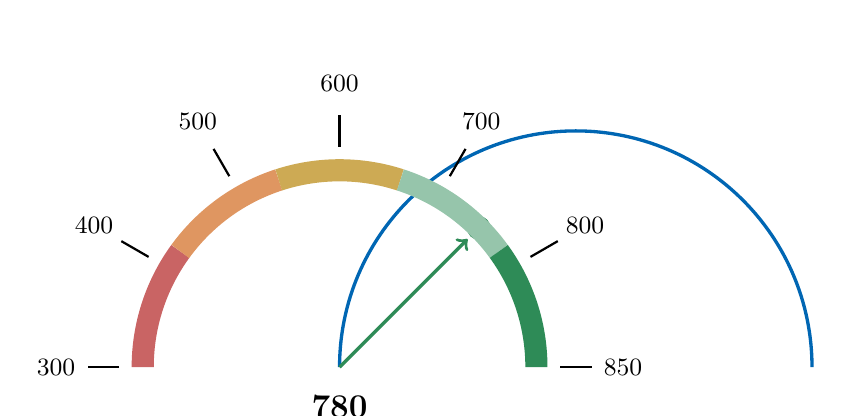
\begin{tikzpicture}
% Credit Score Meter
\draw[very thick, ficoBlue] (0,0) arc (180:0:3cm);
\foreach \angle/\score in {180/300, 150/400, 120/500, 90/600, 60/700, 30/800, 0/850} {
    \draw[thick] (\angle:2.8cm) -- (\angle:3.2cm);
    \node at (\angle:3.6cm) {\small\score};
}
\fill[ficoGreen] (45:2.5cm) circle (0.15cm);
\draw[very thick, ficoGreen, ->] (0,0) -- (45:2.3cm);
\node at (0,-0.5) {\large\bfseries 780};

% Color bands
\draw[line width=8pt, ficoRed!70] (180:2.5cm) arc (180:144:2.5cm);
\draw[line width=8pt, ficoOrange!70] (144:2.5cm) arc (144:108:2.5cm);
\draw[line width=8pt, ficoGold!70] (108:2.5cm) arc (108:72:2.5cm);
\draw[line width=8pt, ficoGreen!50] (72:2.5cm) arc (72:36:2.5cm);
\draw[line width=8pt, ficoGreen] (36:2.5cm) arc (36:0:2.5cm);
\end{tikzpicture}

\vspace{1.5cm}

{\large\itshape A simplified introduction based on the Credit Scoring Primer}\\[2cm]

{\large Credit Rebels Archive}\\[0.5cm]
{\small\url{https://acelogic.github.io/CreditRebelsArchive/}}

\vfill

{\small Last Updated: 2026}

\end{titlepage}

\tableofcontents
\newpage

% ============================================
\section{What is a Credit Score?}
% ============================================

A credit score is a number (300-850) that predicts how likely you are to pay back borrowed money. \textbf{Higher = better.}

\vspace{0.5cm}
\begin{center}
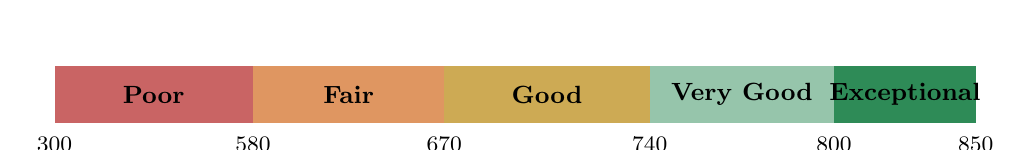
\begin{tikzpicture}[scale=0.9]
% Score ranges as colored bars
\fill[ficoRed!70] (0,0) rectangle (2.8,0.8);
\fill[ficoOrange!70] (2.8,0) rectangle (5.5,0.8);
\fill[ficoGold!70] (5.5,0) rectangle (8.4,0.8);
\fill[ficoGreen!50] (8.4,0) rectangle (11,0.8);
\fill[ficoGreen] (11,0) rectangle (13,0.8);

% Labels
\node at (1.4,0.4) {\small\bfseries Poor};
\node at (4.15,0.4) {\small\bfseries Fair};
\node at (6.95,0.4) {\small\bfseries Good};
\node at (9.7,0.4) {\small\bfseries Very Good};
\node at (12,0.4) {\small\bfseries Exceptional};

% Score numbers
\node at (0,-0.3) {\footnotesize 300};
\node at (2.8,-0.3) {\footnotesize 580};
\node at (5.5,-0.3) {\footnotesize 670};
\node at (8.4,-0.3) {\footnotesize 740};
\node at (11,-0.3) {\footnotesize 800};
\node at (13,-0.3) {\footnotesize 850};
\end{tikzpicture}
\end{center}
\vspace{0.5cm}

\begin{keypoint}
\textbf{Why it matters:} Lenders use your score to decide whether to approve you and what interest rate to charge. A higher score = better rates = less money paid in interest over the life of a loan.
\end{keypoint}

% ============================================
\section{The 5 Things That Affect Your Score}
% ============================================

Think of your score like a pie with 5 slices:

\begin{center}
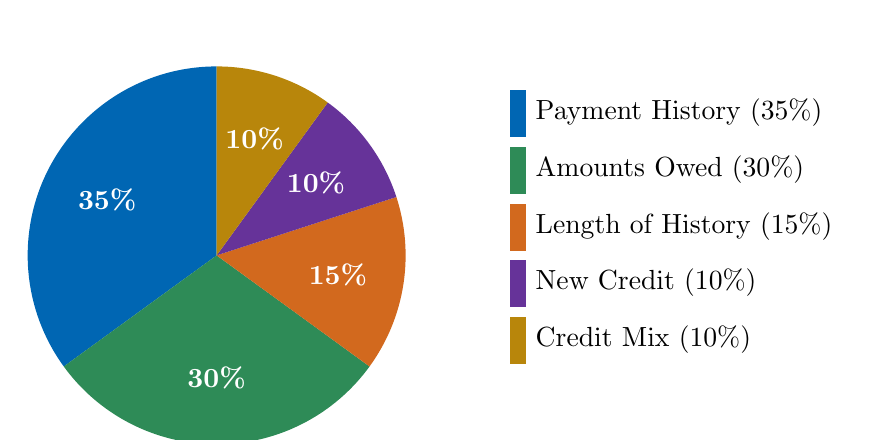
\begin{tikzpicture}[scale=1.2]
% Pie chart
\fill[ficoBlue] (0,0) -- (90:2) arc (90:216:2) -- cycle;
\fill[ficoGreen] (0,0) -- (216:2) arc (216:324:2) -- cycle;
\fill[ficoOrange] (0,0) -- (324:2) arc (324:378:2) -- cycle;
\fill[ficoPurple] (0,0) -- (378:2) arc (378:414:2) -- cycle;
\fill[ficoGold] (0,0) -- (414:2) arc (414:450:2) -- cycle;

% Labels with percentages
\node[white, font=\bfseries] at (153:1.3) {35\%};
\node[white, font=\bfseries] at (270:1.3) {30\%};
\node[white, font=\bfseries] at (351:1.3) {15\%};
\node[white, font=\bfseries] at (396:1.3) {10\%};
\node[white, font=\bfseries] at (432:1.3) {10\%};

% Legend
\node[right] at (3,1.5) {\colorbox{ficoBlue}{\color{white}\small\strut} Payment History (35\%)};
\node[right] at (3,0.9) {\colorbox{ficoGreen}{\color{white}\small\strut} Amounts Owed (30\%)};
\node[right] at (3,0.3) {\colorbox{ficoOrange}{\color{white}\small\strut} Length of History (15\%)};
\node[right] at (3,-0.3) {\colorbox{ficoPurple}{\color{white}\small\strut} New Credit (10\%)};
\node[right] at (3,-0.9) {\colorbox{ficoGold}{\color{white}\small\strut} Credit Mix (10\%)};
\end{tikzpicture}
\end{center}

% --------------------------------------------
\subsection{Payment History (35\%) -- THE BIG ONE}
% --------------------------------------------

\textbf{What it is:} Whether you pay your bills on time.

\begin{warning}
\begin{itemize}[leftmargin=*]
    \item One late payment can drop your score \textbf{50-100+ points}
    \item The more recent the late, the worse the damage
    \item After 7 years, most negative items fall off
\end{itemize}
\end{warning}

\begin{tip}
\textbf{What to do:} Pay at least the minimum on everything, every month, on time. Set up autopay if needed!
\end{tip}

% --------------------------------------------
\subsection{How Much You Owe (30\%)}
% --------------------------------------------

\textbf{What it is:} How much of your available credit you're using (called ``utilization'').

\begin{magicnumber}
Keep your credit card balances below \textbf{9.5\%} of your limits.\\[0.3cm]
Even better: below \textbf{4.5\%} for maximum points on some scorecards.
\end{magicnumber}

\textbf{Example:}
\begin{itemize}[leftmargin=*]
    \item You have a card with a \$1,000 limit
    \item Keep your balance below \$95 when the statement closes
    \item Even better: below \$45 (4.5\%) for maximum points
\end{itemize}

\begin{warning}[title=The ``All Zero'' Trap]
If ALL your cards report \$0 balance, you actually \textbf{LOSE 10-25 points}! Keep a small balance (\$5-20) on ONE card.
\end{warning}

% --------------------------------------------
\subsection{How Long You've Had Credit (15\%)}
% --------------------------------------------

\textbf{What it is:} The age of your credit accounts.

\textbf{Key points:}
\begin{itemize}[leftmargin=*]
    \item Older accounts = better
    \item Don't close old cards, even if you don't use them
    \item Opening new accounts lowers your average age
\end{itemize}

\begin{magicnumber}
\textbf{Important thresholds:}
\begin{itemize}[leftmargin=*]
    \item \textbf{36 months (3 years):} You move to a ``mature'' scorecard
    \item \textbf{90 months (7.5 years):} Believed to be near maximum benefit
\end{itemize}
\end{magicnumber}

% --------------------------------------------
\subsection{New Credit (10\%)}
% --------------------------------------------

\textbf{What it is:} Recent applications for credit.

\textbf{Key points:}
\begin{itemize}[leftmargin=*]
    \item Each application creates a ``hard inquiry''
    \item Inquiries hurt your score for 12 months
    \item They fall off your report after 24-26 months
    \item Multiple inquiries for the same loan type within 14-45 days count as one
\end{itemize}

\begin{keypoint}[title=The Chase 5/24 Rule]
Chase will deny most credit cards if you've opened 5+ cards (any bank) in the last 24 months.
\end{keypoint}

% --------------------------------------------
\subsection{Credit Mix (10\%)}
% --------------------------------------------

\textbf{What it is:} The variety of credit types you have.

\textbf{Good to have a mix of:}
\begin{itemize}[leftmargin=*]
    \item Credit cards (revolving credit)
    \item Auto loan, mortgage, student loans (installment loans)
\end{itemize}

\begin{tip}
\textbf{Ideal ratio:} About 3-4 credit cards to 1 loan.
\end{tip}

% ============================================
\section{Quick Wins to Improve Your Score}
% ============================================

\begin{center}
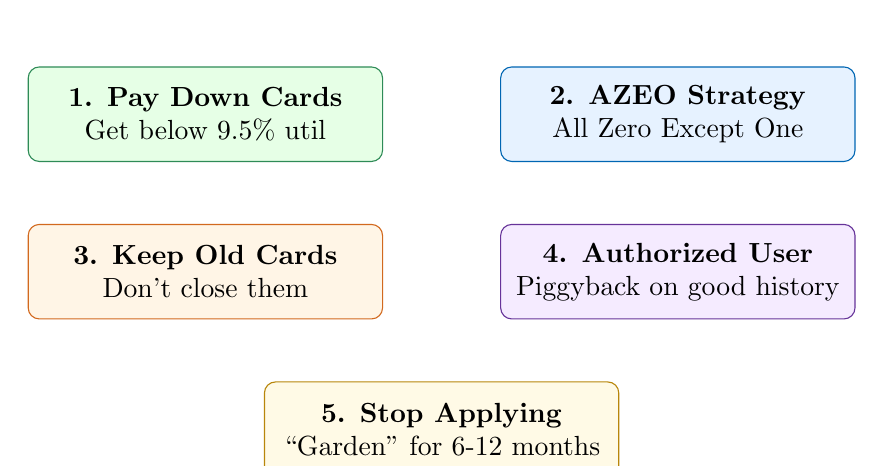
\begin{tikzpicture}
% Quick wins boxes
\node[draw=ficoGreen, fill=lightGreen, rounded corners, minimum width=4.5cm, minimum height=1.2cm, align=center] at (0,4) {\textbf{1. Pay Down Cards}\\Get below 9.5\% util};
\node[draw=ficoBlue, fill=lightBlue, rounded corners, minimum width=4.5cm, minimum height=1.2cm, align=center] at (6,4) {\textbf{2. AZEO Strategy}\\All Zero Except One};
\node[draw=ficoOrange, fill=lightOrange, rounded corners, minimum width=4.5cm, minimum height=1.2cm, align=center] at (0,2) {\textbf{3. Keep Old Cards}\\Don't close them};
\node[draw=ficoPurple, fill=lightPurple, rounded corners, minimum width=4.5cm, minimum height=1.2cm, align=center] at (6,2) {\textbf{4. Authorized User}\\Piggyback on good history};
\node[draw=ficoGold, fill=lightGold, rounded corners, minimum width=4.5cm, minimum height=1.2cm, align=center] at (3,0) {\textbf{5. Stop Applying}\\``Garden'' for 6-12 months};
\end{tikzpicture}
\end{center}

\subsection{1. Pay Down Credit Cards}
Get all cards below 9.5\% utilization. This can boost your score in just one billing cycle.

\subsection{2. AZEO Strategy (All Zero Except One)}
\begin{itemize}[leftmargin=*]
    \item Pay all cards to \$0 before their statement dates
    \item Leave a small balance (\$5-50) on ONE card
    \item This gives you low utilization without the All-Zero penalty
\end{itemize}

\subsection{3. Don't Close Old Cards}
Even if you don't use a card, keeping it open helps your:
\begin{itemize}[leftmargin=*]
    \item Average age of accounts
    \item Total available credit (lowers utilization)
\end{itemize}

\subsection{4. Become an Authorized User}
Ask a family member with a long-standing, well-managed credit card to add you as an authorized user. Their good history can boost your score.

\subsection{5. Stop Applying for Credit}
Every application hurts your score. If you're trying to improve, stop applying for 6-12 months (``gardening'').

% ============================================
\section{Common Myths Debunked}
% ============================================

\begin{mythbox}[title=Myth: ``Checking my own score hurts it'']
\textbf{Truth:} Checking your own score is a ``soft inquiry'' and has NO effect.
\end{mythbox}

\begin{mythbox}[title=Myth: ``I need to carry a balance to build credit'']
\textbf{Truth:} You don't. Pay your full balance each month. Just make sure the statement shows a small balance before you pay it.
\end{mythbox}

\begin{mythbox}[title=Myth: ``Closing cards I don't use will help'']
\textbf{Truth:} It usually hurts. It reduces your available credit and can lower your average account age.
\end{mythbox}

\begin{mythbox}[title=Myth: ``My income affects my score'']
\textbf{Truth:} Income is NOT part of your credit score. Lenders consider it separately.
\end{mythbox}

\begin{mythbox}[title=Myth: ``All credit scores are the same'']
\textbf{Truth:} There are many different scoring models. \fico{} 8 is the most common, but mortgages use \fico{} 2/4/5.
\end{mythbox}

% ============================================
\section{The Scorecards System}
% ============================================

\fico{} doesn't score everyone the same way. You're placed on one of 12 ``scorecards'' based on your profile:

\begin{center}
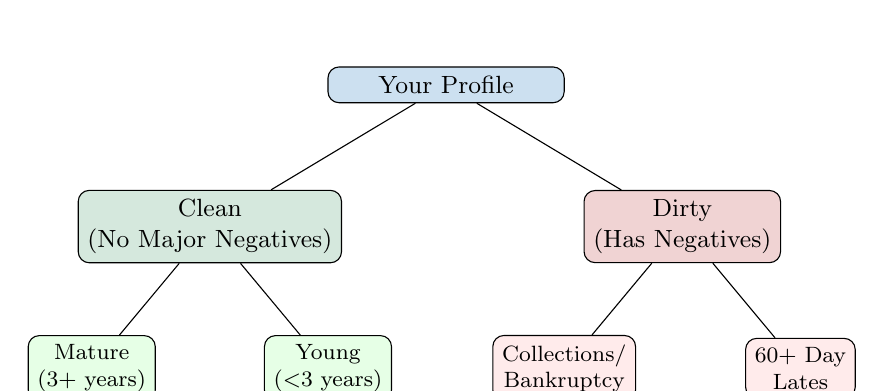
\begin{tikzpicture}[
    level 1/.style={sibling distance=6cm, level distance=1.8cm},
    level 2/.style={sibling distance=3cm, level distance=1.8cm},
    every node/.style={rounded corners, draw, align=center, font=\small}
]
\node[fill=ficoBlue!20, minimum width=3cm] {Your Profile}
    child {node[fill=ficoGreen!20] {Clean\\(No Major Negatives)}
        child {node[fill=lightGreen, font=\footnotesize] {Mature\\(3+ years)}}
        child {node[fill=lightGreen, font=\footnotesize] {Young\\($<$3 years)}}
    }
    child {node[fill=ficoRed!20] {Dirty\\(Has Negatives)}
        child {node[fill=lightRed, font=\footnotesize] {Collections/\\Bankruptcy}}
        child {node[fill=lightRed, font=\footnotesize] {60+ Day\\Lates}}
    };
\end{tikzpicture}
\end{center}

\begin{keypoint}
\textbf{Why this matters:} When you cross a threshold (like hitting 3 years), you change scorecards. This can cause a \textbf{temporary score drop} even though it's actually progress!
\end{keypoint}

% ============================================
\section{Fixing Negative Items}
% ============================================

\subsection{For Accurate Negative Items (you really were late):}
\begin{enumerate}[leftmargin=*]
    \item \textbf{Wait it out} -- Impact decreases over time
    \item \textbf{Goodwill letter} -- Ask the creditor nicely to remove it
    \item \textbf{Use the Saturation Technique} -- Send letters to multiple addresses
\end{enumerate}

\subsection{For Inaccurate Items (errors on your report):}
\begin{enumerate}[leftmargin=*]
    \item \textbf{Dispute with the bureau} (Equifax, Experian, TransUnion)
    \item Provide documentation
    \item They have 30 days to investigate
\end{enumerate}

% ============================================
\section{Your Action Plan}
% ============================================

\begin{center}
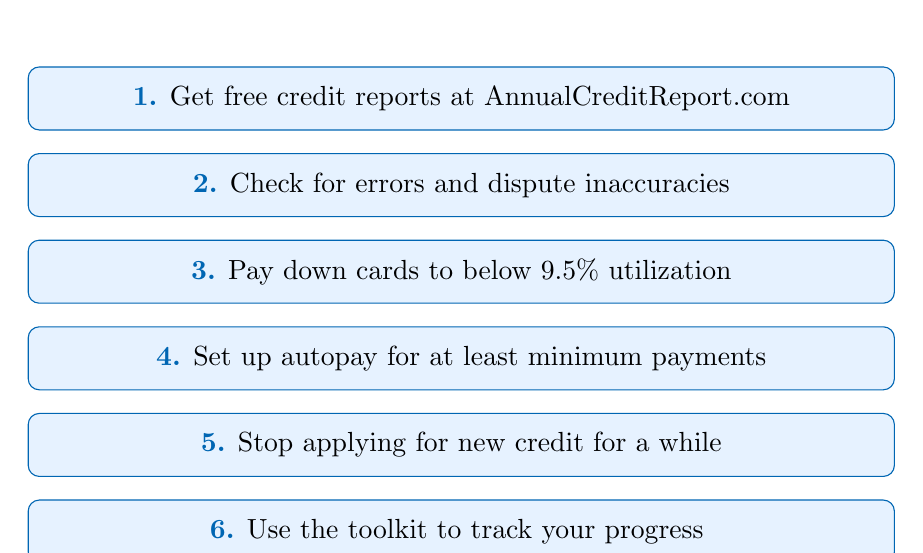
\begin{tikzpicture}
% Numbered steps with arrows
\foreach \i/\text in {
    1/Get free credit reports at AnnualCreditReport.com,
    2/Check for errors and dispute inaccuracies,
    3/Pay down cards to below 9.5\% utilization,
    4/Set up autopay for at least minimum payments,
    5/Stop applying for new credit for a while,
    6/Use the toolkit to track your progress
} {
    \node[draw=ficoBlue, fill=lightBlue, rounded corners, minimum width=11cm, minimum height=0.8cm, align=left] at (0,-\i*1.1) {
        \textbf{\color{ficoBlue}\i.} \text
    };
}
\end{tikzpicture}
\end{center}

% ============================================
\section{Glossary}
% ============================================

\begin{center}
\renewcommand{\arraystretch}{1.4}
\begin{tabular}{>{\bfseries\color{ficoBlue}}l p{10cm}}
\toprule
Term & Meaning \\
\midrule
AAoA & Average Age of Accounts \\
AoOA & Age of Oldest Account \\
AoYA & Age of Youngest Account \\
AZEO & All Zero Except One (strategy) \\
Utilization & Balance $\div$ Credit Limit (as percentage) \\
Hard Inquiry & Credit check when you apply for credit \\
Soft Inquiry & Credit check that doesn't affect score \\
Scorecard & The algorithm group you're assigned to \\
Gardening & Period of not applying for new credit \\
\bottomrule
\end{tabular}
\end{center}

\vspace{1cm}

\begin{center}
\rule{0.5\textwidth}{0.4pt}\\[0.5cm]
{\itshape For the full technical details, see the complete}\\[0.3cm]
{\large\bfseries\href{Credit_Scoring_Primer_v2_Original.pdf}{Credit Scoring Primer v2.0}}
\end{center}

\end{document}
